\section{Quasi-classical approximation}
	The quasi-classical or WKB approximation allows us to solve the Shr\"odinger equation in several cases where it is not possbile to find a direct analytical solution, without resorting to more complex approximations like the perturbation theory.
	
	\subsection{\hl{1D Derivation}}
		\begin{equation}
			-ih\frac{\partial\Psi}{\partial t} = -\frac{\hbar}{2m}\Delta\Psi + U(x)\Psi
		\end{equation}
		Let's search for a solution to the Shr\"odinger equation in the form:
		\begin{equation}
			\Psi = a(x, t)e^{\frac{i}{\hbar}S(x,t)}
		\end{equation}
		Substituting back into the Shr\"odinger equation, we get
		\begin{equation}
			\frac{\partial S}{\partial t} - i \hbar \frac{\partial a}{\partial t} + \frac{a}{2m}(\nabla S)^2 - \frac{i\hbar}{2 m}a\Delta S - \frac{i\hbar}{2m}a\Delta S -\frac{i\hbar}{m}\nabla S \nabla a + Ua = 0
		\end{equation}
		\hl{some voodoo related to Taylor series and $\hbar$}
		\begin{equation}
			\left\{\begin{aligned}
				a \frac{\partial a}{\partial t} + \frac{a}{2m}(\nabla S)^2 + Ua= 0\\
				-i\hbar \left(\frac{\partial a}{\partial t} + \frac{1}{2m}a\frac{\partial^2S}{\partial x^2} + \frac{1}{m}\nabla S\nabla a\right)= 0
			\end{aligned}\right.
		\end{equation}
		We know that if the hamiltonian of the system, $\hat{H}$, is time-independent, then the solutions to the Shr\"odinger equation are in the form of $\Psi = a e ^ {-\frac{iE}{\hbar}t}$, which means that:
		\begin{align}
			\Psi = a e ^ {-\frac{iE}{\hbar}t} =& a(x, t)e^{\frac{i}{\hbar}S(x,t)} \\
			S =& Et + S_0(x) \\
			a(x, t) =& a(x)
		\end{align}
		and
		\begin{equation}
			\left\{\begin{aligned}
				\frac{1}{2m}(\nabla S_0)^2 + U = E \\
				\hbar\left(\frac{a}{2m}\Delta S_0 + \frac{1}{m}\nabla S_0\nabla a\right) = 0
			\end{aligned}\right.
		\end{equation}		
		Because we are solving for a 1D case,
		\begin{align}
			\frac{1}{2m}\left(\frac{\partial S_0}{\partial x}\right)^2 =& E - U\\
			\frac{\partial S_0}{\partial x} =& \sqrt{2m(E-U)}\\
			S_0 =& \int_{a_0}^{x}\sqrt{2m(E-U)}dx
		\end{align}	
	
		\begin{align}
			\frac{a}{2m} \frac{\partial^2 S_0}{\partial x^2} + \frac{1}{m}\frac{\partial S_0}{\partial x}\frac{\partial a}{\partial x} =& 0 |\times a\\
			\div\left(a^2 \frac{\nabla S_0}{m}\right) = 0, \quad \nabla S_0 = \sqrt{2m(E-U)} =& p \Rightarrow\\
			\frac{a^2\nabla S_0}{m} = \frac{a^2p}{m} =& const \\
			a^2p =& const \rightarrow \\
			a =& \pm \frac{c}{\sqrt{p}}
		\end{align}
		Which gives us the final form of $\Psi$, where $c_1, c_2$ are normalization constants:
		\begin{equation}
			\Psi = \frac{c_1}{\sqrt{p}}\exp(\frac{i}{\hbar}\int_a^x pdx) + \frac{c_2}{\sqrt{p}}\exp(-\frac{i}{\hbar}\int_a^x pdx)
		\end{equation}
		\subsubsection{Applicability}
			When we did the \hl{magic voodoo that I missed in class}, we took for granted that 
			\begin{equation}
				\frac{a}{2m}(\nabla S_0)^2 \gg \frac{i\hbar}{2m}\Delta S_0
			\end{equation}
			Which, considering that $\nabla S_0 = p$ and introducing the de Broglie wavelength, $\lambda_B = \frac{\hbar}{p}$ is equivalent to:
			\begin{align}
				\frac{a}{2m}(\nabla S_0)^2 \gg& \frac{i\hbar}{2m}\Delta S_0 \\
				frac{p^2} \gg& i\hbar\frac{\partial p}{\partial x} \\ 
				\frac{\hbar}{p^2}\left|\frac{dp}{dx}\right| \ll& 1 \\
				\left|\frac{d\lambda_B}{dx}\right| \ll&  1 \Leftrightarrow\\
				\left|U(x)\right| \gg& \lambda_B
			\end{align}
			Which means that the quasi-classical approximation is applicable when the potential varies slowly relative to the de Broglie wavelength of the partical in the potential.
	
	\subsection{Problems}
		\subsubsection{Exponential potential}
			\begin{figure}[!h]
				\centering
				\begin{tikzpicture}[scale=1,cap=round,>=latex]
\draw [<->] (0, 3) -- (0, 0) -- (7, 0);
\node [left] at (0, 3) {$U$};
\node [below] at (7, 0) {$x$};

\draw [line width=1.5] (0, 0) -- (2, 0) -- (2, 3/2);
\draw[domain=2:7,smooth,line width=1.5, variable=\x] plot ({\x},{3/\x});

\node [below] at (2, 0) {$a$};

\end{tikzpicture}
				\caption{Exponentially decaying potential barrier}
			\end{figure}
			For a potential barrier:
			\begin{align}
				U(x) = \left\{ \begin{aligned}
					0,\quad x < a \\
					\frac{\alpha}{x},\quad x > a
				\end{aligned}
				\right. \\
			\end{align}
			and a particle with $E > 0$, what are the reflection and transmission coefficients?
			
		\subsubsection{Hemisphere potential}
			\begin{figure}[!h]
				\centering
				\begin{tikzpicture}cap=round,>=latex]
	\begin{axis}[grid=none,
	axis x line=middle,
	axis y line=left,	
	enlargelimits,
	xtick={-1,0,1},
	xticklabels={$-a$, $0$, $a$},
	ytick={1},
	yticklabels={$U_0$},
	domain=-1.2:1.2
	]
	
	\addplot[no markers, line width=1.5, samples=50, domain=-1:1] {cos(deg(pi*x/2))};
	\end{axis}								
\end{tikzpicture}
				\caption{Hemisphere potential barrier}
			\end{figure}
			For a potential barrier:
			\begin{align}
				U(x) = U_0 \cos(\frac{\pi}{2a}x), \quad -a \leq x \leq a
			\end{align}
			and a particle with $E > 0$, what are the reflection and transmission coefficients?
		\subsubsection{Minimal transistor size}
			\begin{figure}[!h]
				\centering
				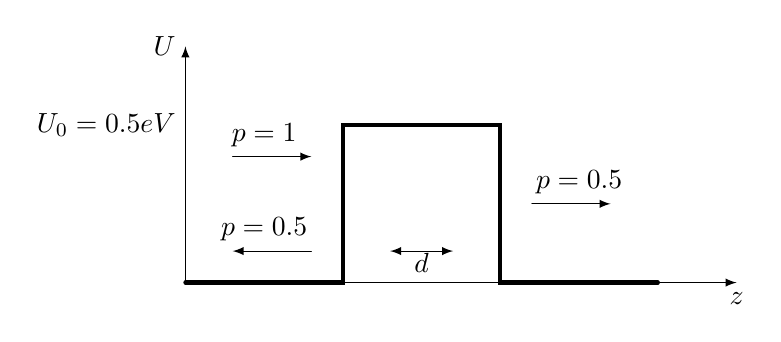
\begin{tikzpicture}[scale=2,cap=round,>=latex]
	\draw [<->] (-2, 1.5) -- (-2, 0) -- (1.5, 0);
	\node [left] at (-2, 1.5) {$U$};
	\node [below] at (1.5, 0) {$z$};
	
	\draw [line width=1.5] (-2, 0) -- (-1, 0) -- (-1, 1) -- (0, 1) -- (0, 0) -- (1, 0);
	
	\node [above] at (-0.5, 0) {$d$};
	\draw [<->] (-0.7, 0.2) -- (-0.3, 0.2);	
	
	\node [left] at (-2, 1) {$U_0 = 0.5\si{eV}$};

	\draw [->] (-1.7, 0.8) -- (-1.2, 0.8);
	\node [above] at (-1.5, 0.8) {$p = 1$};
		
	\draw [<-] (-1.7, 0.2) -- (-1.2, 0.2);
	\node [above] at (-1.5, 0.2) {$p = 0.5$};

	\draw [->] (0.2, 0.5) -- (0.7, 0.5);	
	\node [above] at (0.5, 0.5) {$p = 0.5$};
												
\end{tikzpicture}
				\caption{Model transistor}
			\end{figure}
			
			\begin{align}
				m_{el} \approx& 0.3 m_0 \\
				m_0 \approx& 10^{-30}\si{kg} \\
				p =& |\Psi|^2
			\end{align}			
			
			Calculate the size of a quantum barrier at which an electron's probability of tunneling through is equal to $0.5$ using the quasi-classical approach, and compare it to the exact solution.
		
		\subsubsection{Classical limit*}	
			For a potential $U(x)$ that possesses a certain number of bound states with energies $E_n$, in the limit $n\rightarrow\infty$, we transition into classical mechanics. 
			
			How does $\Delta E = E_{n+1}-E_n$ change for $n\rightarrow\infty$?
